
\section{Architecture Integration}

\subsection{Model Support Matrix}

\begin{table}[H]
\centering
\small
\begin{tabular}{lllll}
\toprule
\textbf{Architecture} & \textbf{Attention} & \textbf{Nested?} & \textbf{RoPE?} & \textbf{GQA?} \\
\midrule
DistilBERT & \texttt{MultiHeadSelfAttention} & No & No & No \\
RoBERTa & \texttt{BertSelfAttention} & Yes & No & No \\
GPT-2 & \texttt{GPT2Attention} & No & No & No \\
Qwen3.5 & \texttt{Qwen3Attention} & No & Yes & Yes \\
\bottomrule
\end{tabular}
\end{table}

\subsection{Weight Transfer}

\subsubsection{GPT-2 (Conv1D)}

\begin{lstlisting}
c\_w = src.c\_attn.weight.data
if is\_conv1d:
    c\_w = c\_w.t()
q\_w, k\_w, v\_w = c\_w.chunk(3, dim=0)
\end{lstlisting}

\subsubsection{RoBERTa (Nested)}

\begin{lstlisting}
q\_w = src.self.query.weight.data
k\_w = src.self.key.weight.data
v\_w = src.self.value.weight.data
o\_w = src.output.dense.weight.data
\end{lstlisting}

\subsubsection{DistilBERT (Flat)}

\begin{lstlisting}
q\_w = src.q\_lin.weight.data
k\_w = src.k\_lin.weight.data
v\_w = src.v\_lin.weight.data
o\_w = src.out\_lin.weight.data
\end{lstlisting}

\subsection{Gate Initialization}

\begin{lstlisting}
self.gate = nn.Linear(self.dim, self.num\_heads)
self.gate.bias.data.fill\_(gate\_init\_bias)  # default 1.8
\end{lstlisting}

With \texttt{gate\_init\_bias = 1.8}: $\sigma(1.8) \approx 0.86$. The gate initially 
favors the short (sliding-window) branch.

\subsection{Preservation Gate Initialization}

\begin{lstlisting}
self.output\_gate = nn.Parameter(torch.tensor(2.0))
\end{lstlisting}

At initialization: $\alpha = \sigma(2.0) \approx 0.88$.

\subsection{RoPE Extraction}

For Qwen:

\begin{lstlisting}
if position\_embeddings is not None:
    cos, sin = position\_embeddings
    q, k = apply\_rotary\_pos\_emb(q, k, cos, sin)
elif self.rotary\_emb is not None:
    try:
        cos, sin = rotary\_module(q, seq\_len=L)
    except Exception:
        try:
            cos, sin = rotary\_module(q, pos\_ids)
        except Exception:
            cos, sin = None, None
\end{lstlisting}

\subsection{GQA Support}

\begin{lstlisting}
if self.kv\_repeat \textgreater{} 1:
    k = repeat\_kv(k, self.kv\_repeat)
    v = repeat\_kv(v, self.kv\_repeat)
\end{lstlisting}

\subsection{Injection}

\textbf{Algorithm 2:} Inject GoldFinch-AHN
\begin{lstlisting}
1: new $\leftarrow$ GoldFinchAHNBlock(config, old=old\_attn)
2: if copy\_weights fails: return None
3: if   has .attention.self:
4:      .attention.self $\leftarrow$ new; is\_nested $\leftarrow$ True
5: elif   has .attention:
6:      .attention $\leftarrow$ new
7: elif   has .self:  .self $\leftarrow$ new; is\_nested $\leftarrow$ True
8: elif   has .attn:  .attn $\leftarrow$ new
9: return new
\end{lstlisting}

\subsection{Common Pitfalls}

\subsubsection{The `GatedDeltaNetLayer` is a Linear Projection}

The name is misleading. The class does not implement a recurrent mechanism.

\subsubsection{`output\_scale` Redundancy}

\texttt{LoRALinear} has \texttt{self.output\_scale = nn.Parameter(torch.ones(1))} applied 
at the end of \texttt{forward}. Additionally, \texttt{GoldFinchAHNBlock} has its own 
\texttt{self.output\_scale}. \textbf{Double scaling} can occur.

\subsubsection{Gate Mean Over Heads}

The gate is computed per-head but then \textbf{mean-pooled}:

\begin{lstlisting}
gate = torch.sigmoid(self.gate(x)).mean(dim=-1, keepdim=True)
\end{lstlisting}

This destroys per-head differentiation. The resulting \texttt{gate} has shape 
\texttt{(B, L, 1)} -- a single scalar per token, applied uniformly across all heads.

\subsubsection{Preservation Gate Means High Residual}

With $\alpha \approx 0.88$, only ~12\% of the block's output reaches the 
next layer. This makes the block \textbf{conservative}.

\subsection{Registry}

\begin{lstlisting}
@ATTENTION\_REGISTRY.register("goldfinch\_ahn")
@ATTENTION\_REGISTRY.register("goldfinch")
class GoldFinchAHNBlock(BaseAttention):
    ...
\end{lstlisting}



\begin{figure}[H]
\centering
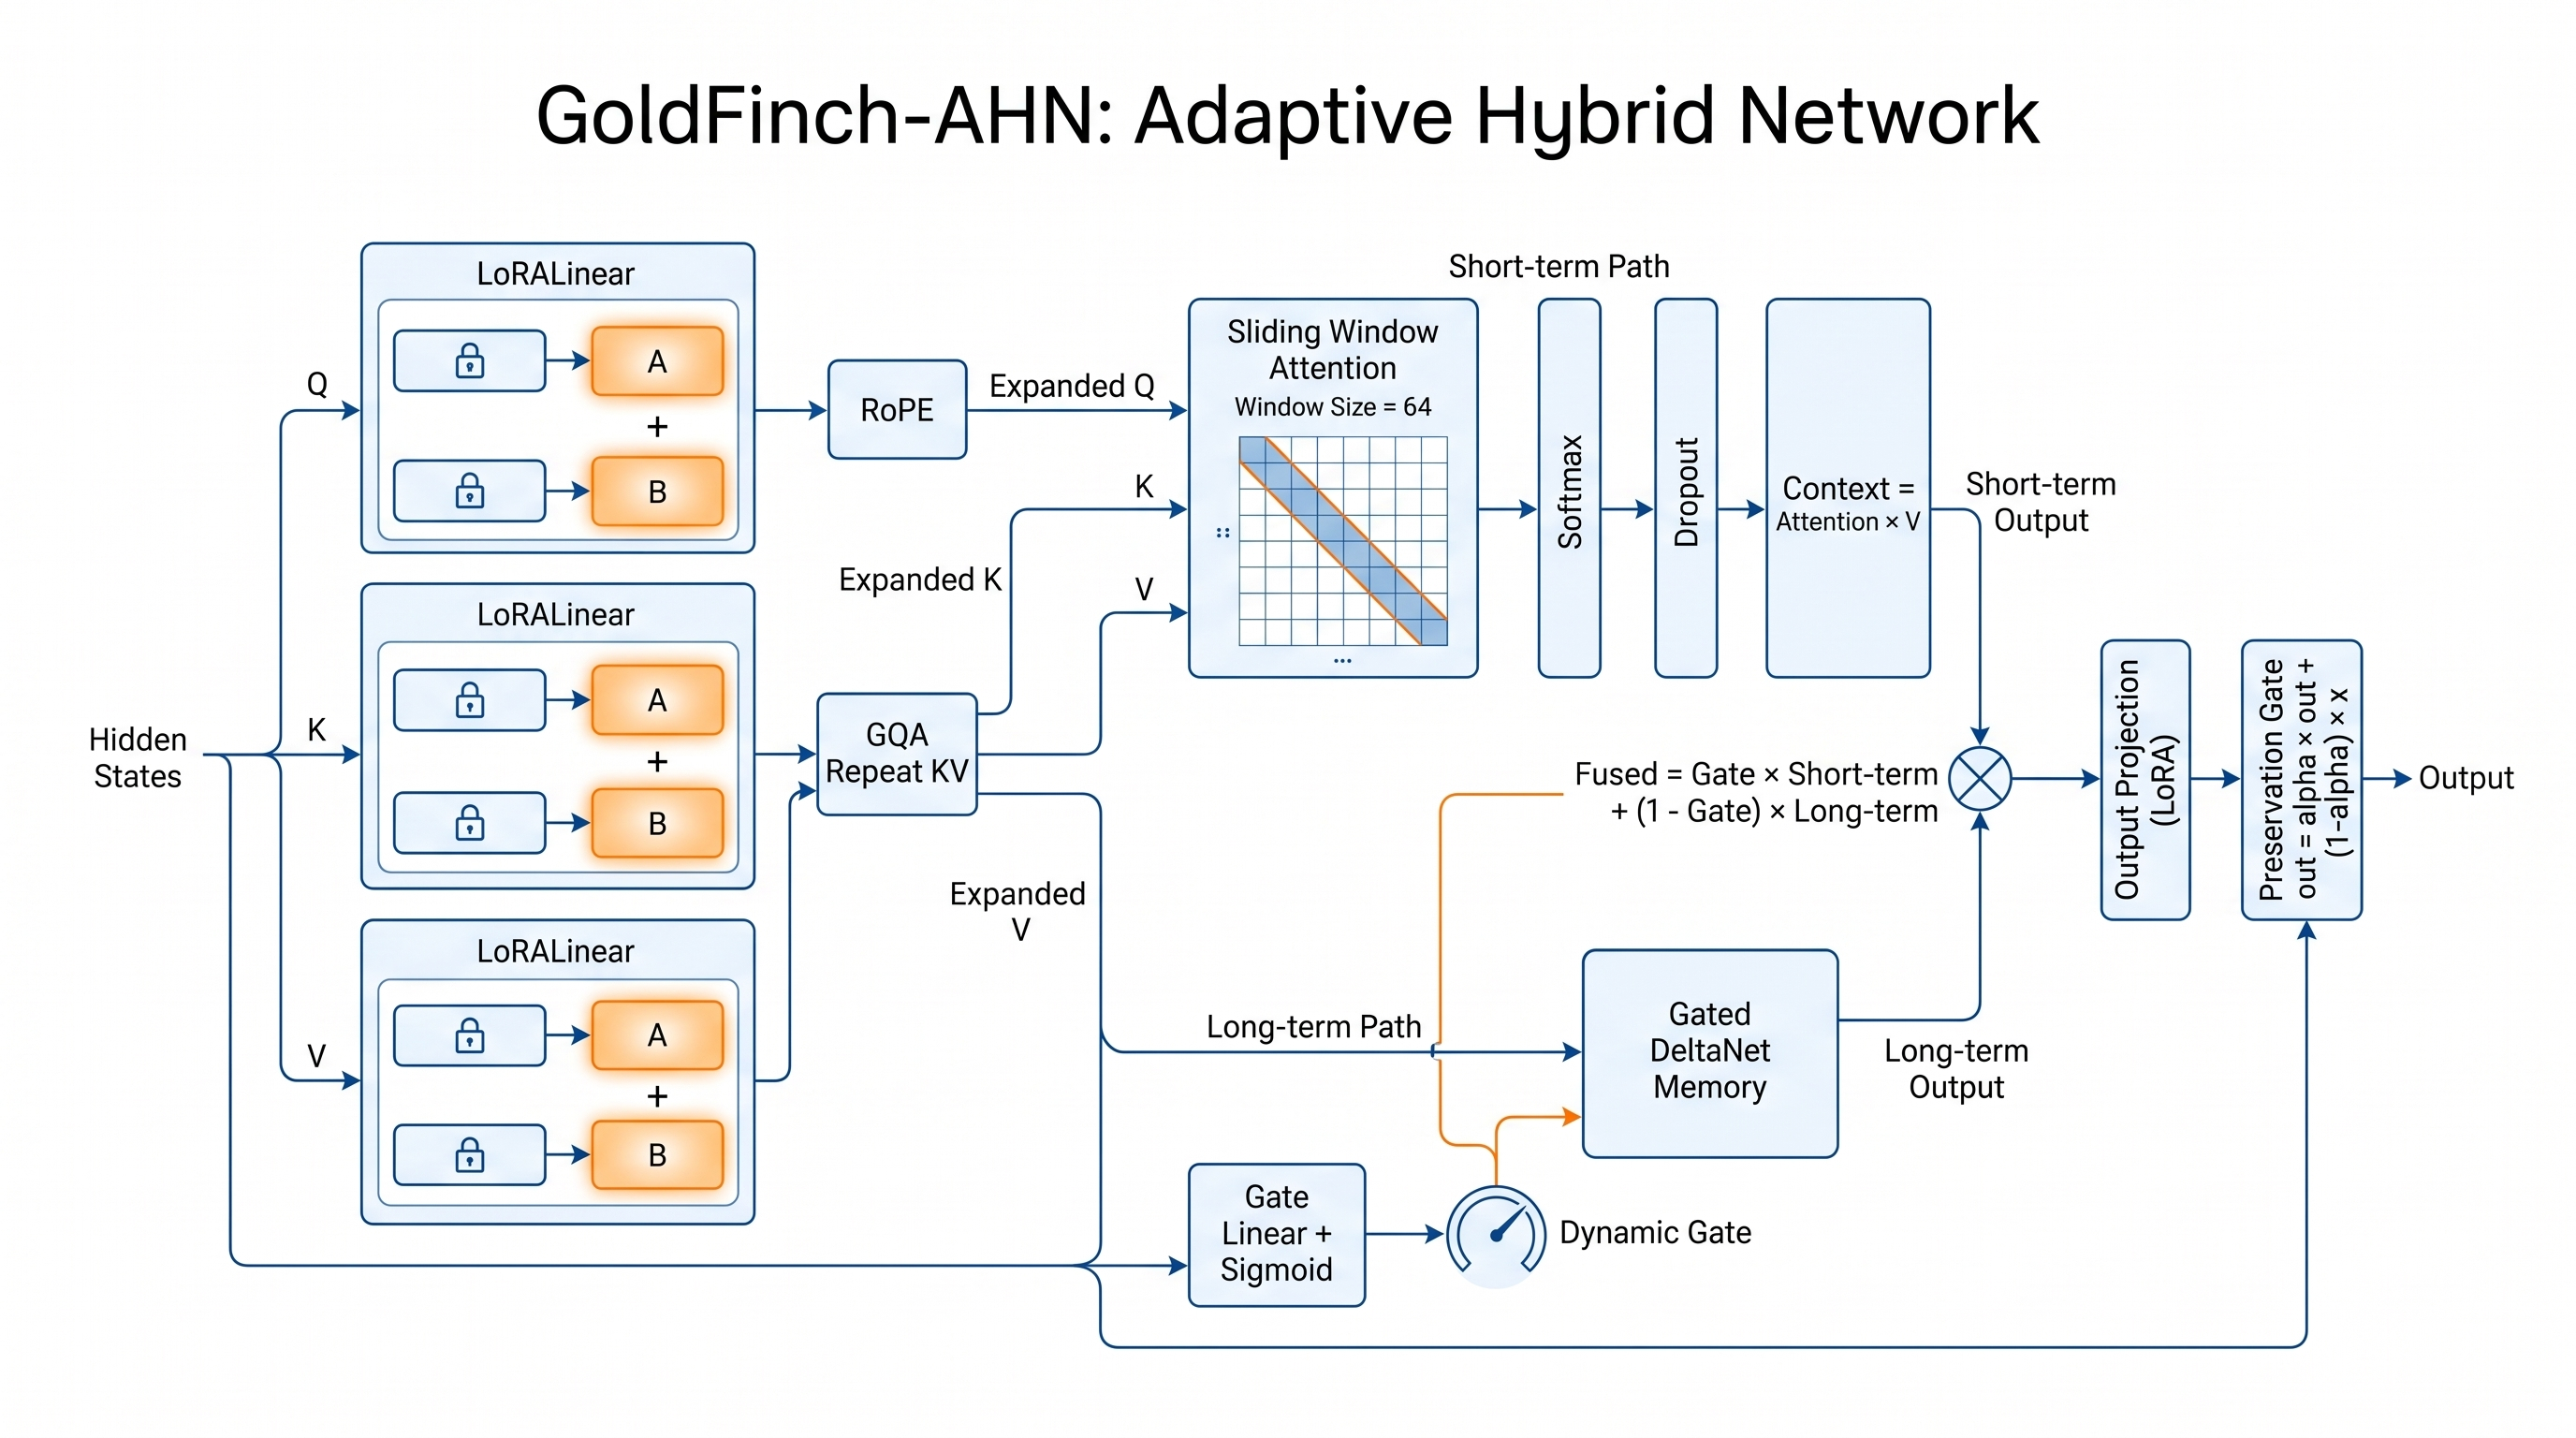
\includegraphics[width=\linewidth]{figures/architecture.jpeg}
\caption{High-level architectural diagram of goldfinch\_ahn.}
\label{fig:arch\_goldfinch-ahn}
\end{figure}

